\documentclass[11pt,a4paper]{ctexart}
\usepackage{geometry}
\usepackage{amsmath}
\geometry{left=2.5cm, right=2.5cm, top=3cm, bottom=3cm}
\usepackage{tcolorbox}
\usepackage{xcolor}
\usepackage{enumitem}
\usepackage{subfigure}

% 自定义高亮思考框样式
\tcbset{
    reflectionbox/.style={
        colback=yellow!10!white,
        colframe=orange!80!black,
        fonttitle=\sffamily\bfseries,
        title={ 独立思考与深度反思 (Highlight)},
        boxrule=1pt,
        arc=4pt,
        left=2mm, right=2mm, top=2mm, bottom=2mm
    }
}

\title{\vspace{-2cm}\textbf{多 Agent 资源博弈管理系统实践报告}}
\author{231240045 杨俊炜}
\date{2026/5/21}

\begin{document}
\maketitle
\vspace{-1.5cm}

\section{问题背景与系统目标}
针对在家中多台旧设备上部署计算任务的场景，本实践设计并实现了一个基于多智能体（Multi-Agent）的资源博弈调度系统。系统包含一个核心的 \textbf{Master Agent} 和多个分布式运行的 \textbf{Worker Agent}，旨在通过模拟《星际争霸》等游戏中的微观资源管理机制，实现计算任务的高效分配与老旧设备的功耗平衡。

系统的核心调度逻辑建立在\textbf{“饥饿感”与“电费 Token”机制}之上：
\begin{itemize}[leftmargin=*]
    \item 当某台设备的 Token 不足（低于抢占阈值 10）时，将触发“饥饿”状态。此时设备无法接取高收益任务，必须通过执行低功耗打工任务（如待机散热降温）来积攒 Token。
    \item 当设备的 Token 充足时，Master Agent 会根据全局策略，向其分配“大型 C++ 编译”或“LLM 推理”等重负载任务。在执行过程中，节点需支付相应的 Token 作为资源成本。
    \item 为保障物理设备的安全，Master Agent 实施严格的实时监控。一旦发现某设备温度过高（如超过 $85^\circ\text{C}$）或 CPU 持续满载，将执行严厉的 Token 扣除惩罚机制。
\end{itemize}

\section{实践过程与系统架构设计}
本系统基于 Python 语言开发，并引入了 \textbf{Ray 分布式计算框架} 来构建底层集群拓扑。主要模块设计如下：
\begin{enumerate}[leftmargin=*]
    \item \textbf{Worker 节点架构：}封装了设备的物理运行状态，包括 CPU 占用率、温度指标、Token 余额以及系统累积得分。为 Worker 设计了 \texttt{run\_low\_power\_task()} 与 \texttt{run\_heavy\_task()} 两种核心行为接口，通过模拟不同的运行耗时、发热特征及耗电曲线，展现出鲜明的状态转移逻辑。
    \item \textbf{Master 调度中枢设计：}作为全局宏观调控中心，初始化时在 Ray 集群中部署多个独立的 Worker Actor 进程。在系统运行时，Master 采用回合制（Rounds）循环执行调度：包括同步拉取所有节点状态、执行过热惩罚判定、基于当前 Token 分布进行任务抢占与下发。
\end{enumerate}

\section{实践中遇到的困难与解决办法}

\subsection{挑战 1：单机环境下的分布式调度与状态隔离}
\textbf{实践困难：} 在实验初期的代码编写阶段，首要难点是如何在单台个人笔记本电脑上，模拟出多台物理隔离的老旧电脑并发运行，并对它们的状态进行统一、非阻塞的监控与追踪。传统的 Python 多线程/多进程库编写繁琐且难以实现跨节点的对象状态同步。

\textbf{解决办法：} 放弃了底层并发库，选择引入成熟的 \textbf{Ray 框架} 实现分布式调度。通过将 \texttt{WorkerAgent} 类加上 \texttt{@ray.remote} 装饰器，直接将各设备实例化为 Ray 集群中独立的 Actor 进程。Master 节点只需通过远程方法调用（RPC）即可下发指令，并通过返回的对象引用（Object Ref）统一同步节点状态。

\begin{tcolorbox}[reflectionbox]
多 Agent 系统的设计精髓在于“去中心化的执行”与“中心化的监管”相分离。引入 Ray 框架不仅完美解决了本地进程隔离与异步通信的痛点，更为项目未来向真实的跨机器分布式集群（如局域网内互联的废旧笔记本）平滑迁移奠定了基础。这种“单机模拟验证，无缝拓展至集群”的工程设计思维，是构建高可用分布式架构的最佳实践原则。
\end{tcolorbox}

\subsection{挑战 2：高真实度模拟与资源博弈生态平衡}
\textbf{实践困难：} 最初编写逻辑时，任务对 Token 的消耗、赚取数值以及温度的增加幅度均采用了定值（固定魔法数值）。多次运行后发现，模拟结果过于线性、刻板，节点状态呈现机械的周期性循环，完全脱离了老旧设备在真实运行大型编译或大模型推理时的发热随机性与负载波动。

\textbf{解决办法：} 针对不同负载类型进行精细化与随机化重构。考虑到现实场景，我为“LLM 推理”和“大型 C++ 编译”设计了不同的资源指纹：LLM 推理的 Token 消耗更大（10）、温度跃升更剧烈（增加 $20 \sim 30^\circ\text{C}$）；而大型编译耗能略小（8）。此外，所有的状态变化数值均使用 \texttt{random.uniform} 或 \texttt{random.randint} 生成动态随机浮动区间的变量，以模拟真实物理环境。

\begin{tcolorbox}[reflectionbox]
真实物理硬件的瓶颈往往是非线性的黑盒。旧设备的散热能力衰减、后台进程抢占等情况，必然伴随着随机波动。将死板的定值模型改为基于硬件特性的“噪声区间”，彻底激活了博弈机制：有些设备可能因随机的温度暴增而直接触发“过热熔断”惩罚（扣除 15 Token），被迫长期陷入“饥饿打工”状态无法自拔。引入这种底层的“物理不可靠性”，使得 Master Agent 的调度策略面临更真实的博弈考验，也让整个系统的资源争夺生态变得丰富而不可预测。
\end{tcolorbox}

\subsection{挑战 3：回合制状态同步与异步执行的时序冲突}
\textbf{实践困难：} 随着模拟环境加入了随机耗时，不同进程的 Worker 节点任务执行步调产生差异。由于代码是异步调用的，导致 Master 在回合末尾拉取状态时发生了严重的“时序错位”——可能取到了上一回合尚未更新的旧数据。结算日志呈现出状态混乱，导致惩罚与奖励的逻辑判断发生误判，破坏了调度的公平性。

\textbf{解决办法：} 在 Master 的调度回合（Round）末尾，强制引入了时间与状态的“同步屏障”（Barrier）机制。在下发完所有异步任务后，首先使用 \texttt{time.sleep()} 让主进程短暂挂起等待执行完毕；最核心的改动是，在获取所有节点状态时，强制使用 \texttt{ray.get()} 的阻塞特性，确保所有 Actor 的远程状态均已正确更新并返回后，再打印本回合结算面板，随后进入下一轮的博弈。

\begin{tcolorbox}[reflectionbox]
这是分布式系统中经典的“一致性与并发性”冲突。在追求 Agent 并发执行效率的同时，必须在关键的业务节点（即本系统的每一回合结算点）建立强约束的“状态快照”。采用 \texttt{ray.get()} 阻塞拉取，虽然牺牲了极少量的主进程等待时间，却换来了整个博弈系统在逻辑调度上的绝对一致性与正确性。若无状态的一致性保证，基于此产生的所有 Token 扣除和奖励都将失去合法依据，整个多智能体系统将陷入混沌。因此，在特定环节“以局部同步保全局一致”，是复杂调度系统不可或缺的设计妥协。
\end{tcolorbox}

\section{运行结果与讨论}
通过在终端运行 10 个回合的集群调度测试（5 台 Worker 节点），系统成功呈现了预期的资源博弈与动态调控效果。实验日志清晰地展示了以下三个阶段的演化：

\subsection{初始冷启动与资源积累（回合 1-2）}
在系统启动初期，所有节点的初始 Token 均为 0。Master Agent 成功识别到集群处于整体“饥饿状态”，强制所有节点执行低功耗打工任务。在这两个回合中，各节点 CPU 占用率维持在 20\% 以下，温度保持在 $30^\circ\text{C}$ 左右的安全基线，并成功将 Token 积累至抢占阈值（10 Token）以上。

\subsection{高负载抢占与温度飙升（回合 3-6）}
进入回合 3 后，Token 充足的节点开始“挥霍”资源，大规模抢占 LLM 推理与大型 C++ 编译任务。日志显示，执行重负载任务的节点 CPU 瞬间飙升至 90\% 以上，温度随之剧烈上升（如 Node-1 温度达到 $56.67^\circ\text{C}$）。在回合 6 中，高真实度的随机波动带来了极端情况：Node-3 在执行重载任务后，温度失控飙升至 $102.62^\circ\text{C}$，触发了 Master 的安全红线。

\subsection{散热困境与长尾惩罚效应（回合 7-10）}
由于 Master 的过热惩罚机制（扣除 15 Token），部分过热节点（如 Node-1 和 Node-3）不仅 Token 被清零，且由于物理散热需要时间，在后续的低功耗打工回合中，其温度依然高于 $85^\circ\text{C}$（例如 Node-3 在回合 8 仅有 15.04\% 的 CPU 占用，但温度仍高达 $92.24^\circ\text{C}$）。这导致它们连续遭遇“过热或满载”警告，陷入了长期的“零 Token + 强制休眠散热”的困境。而同时期散热良好的节点（如 Node-4、Node-5）则在回合 10 重新攒够 Token，再次接取了高收益任务。

\begin{figure}[htbp]
\centering
\subfigure[1-2]
{
    \begin{minipage}[b]{.3\linewidth}
        \centering
        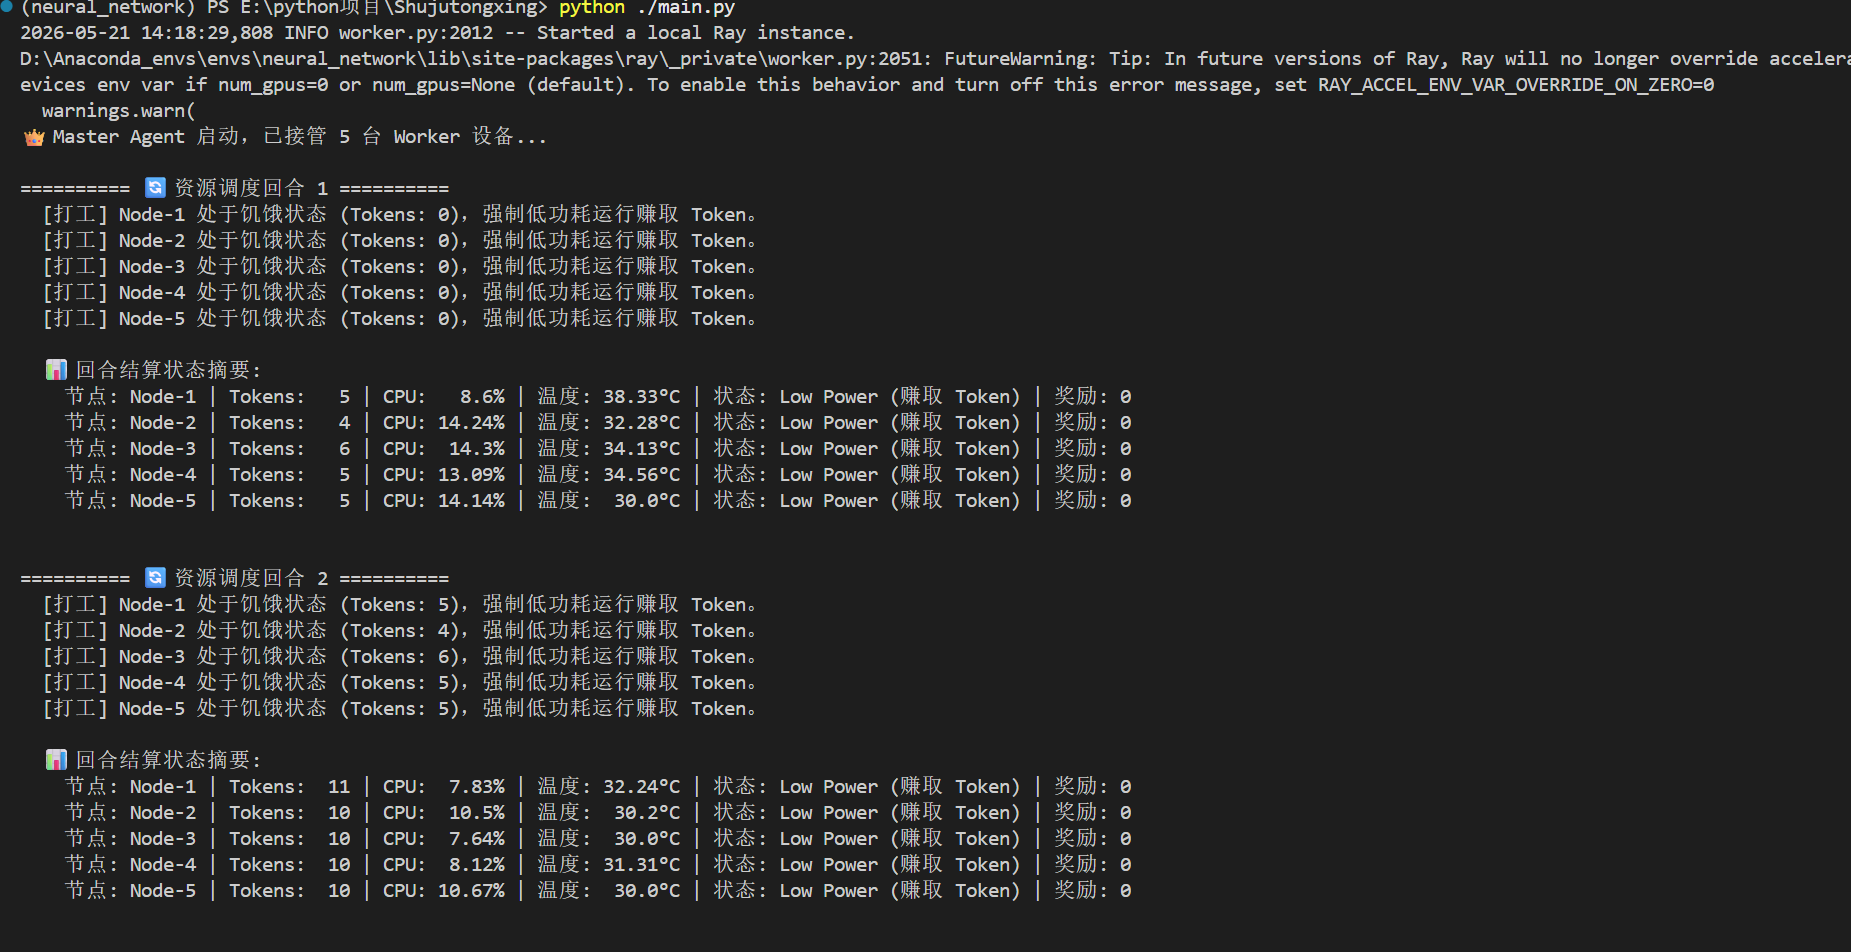
\includegraphics[scale=0.2]{1-2.png}
    \end{minipage}
}
\subfigure[3-4]
{
 	\begin{minipage}[b]{.3\linewidth}
        \centering
        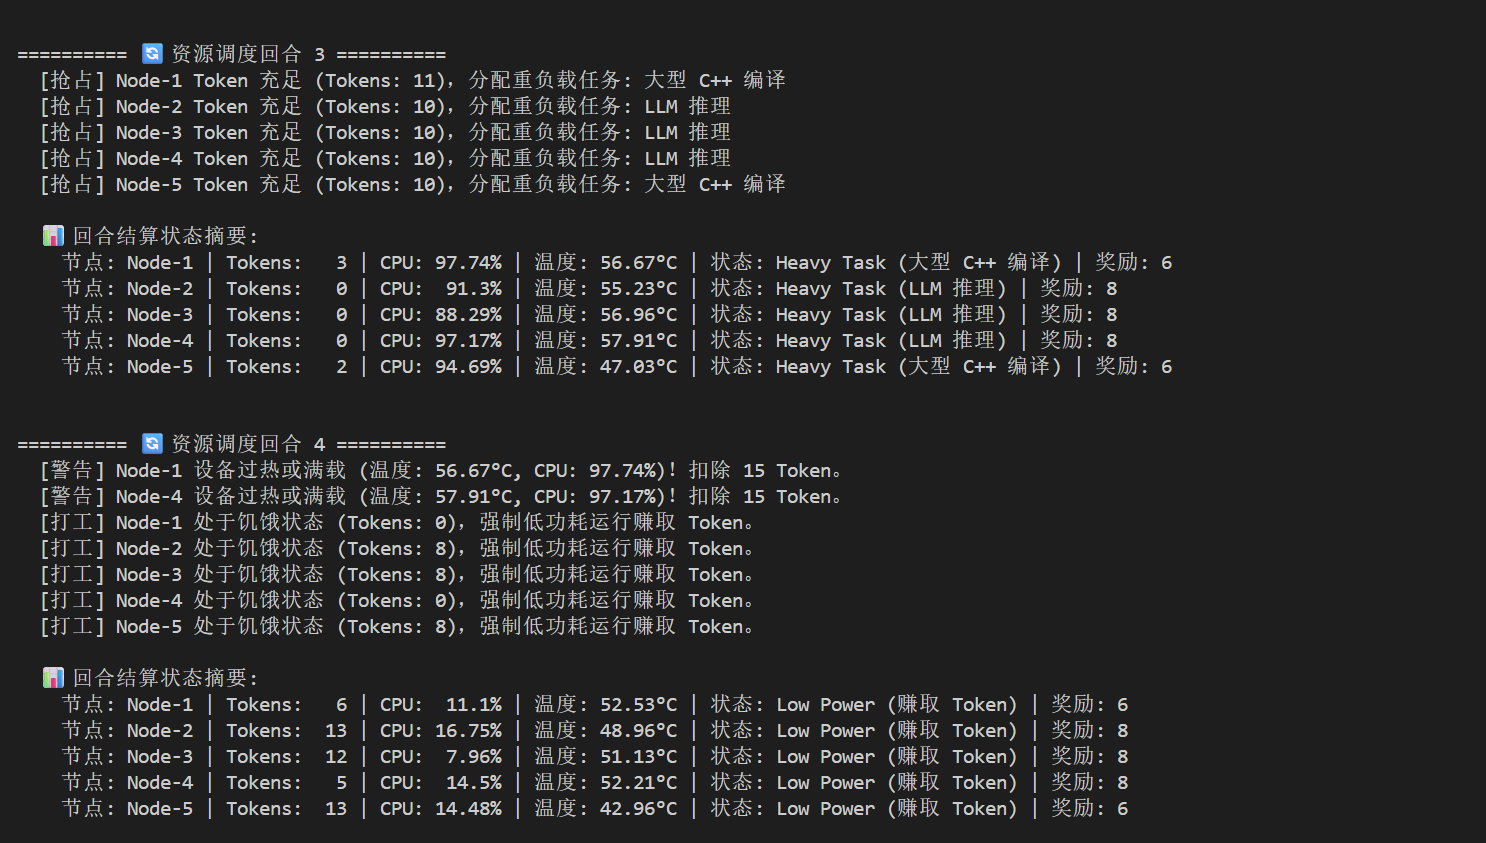
\includegraphics[scale=0.2]{3-4.png}
    \end{minipage}
}
\subfigure[5-6]
{
 	\begin{minipage}[b]{.3\linewidth}
        \centering
        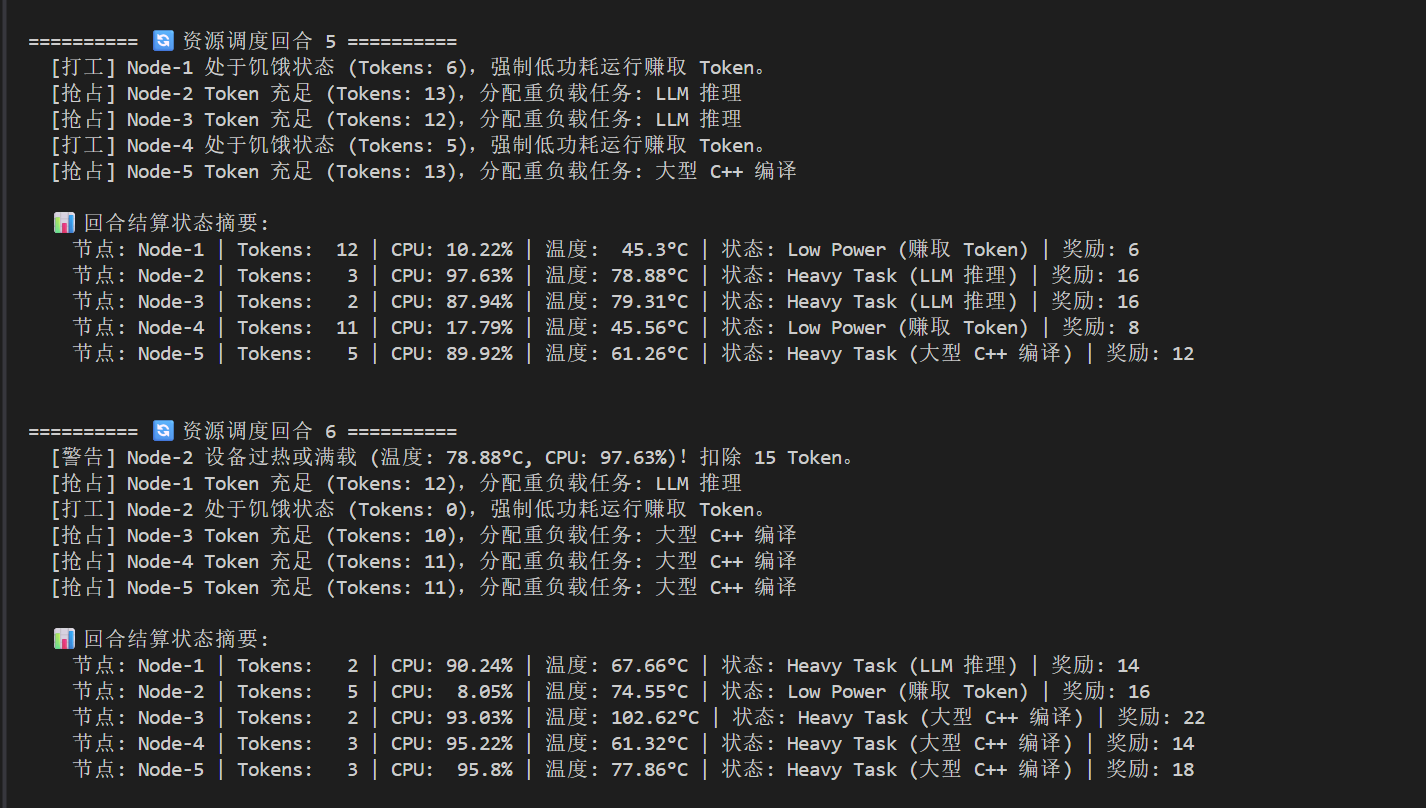
\includegraphics[scale=0.2]{5-6.png}
    \end{minipage}
}
\caption{1-6回合}
\end{figure}

\begin{figure}[htbp]
\centering
\subfigure[7-8]
{
    \begin{minipage}[b]{.3\linewidth}
        \centering
        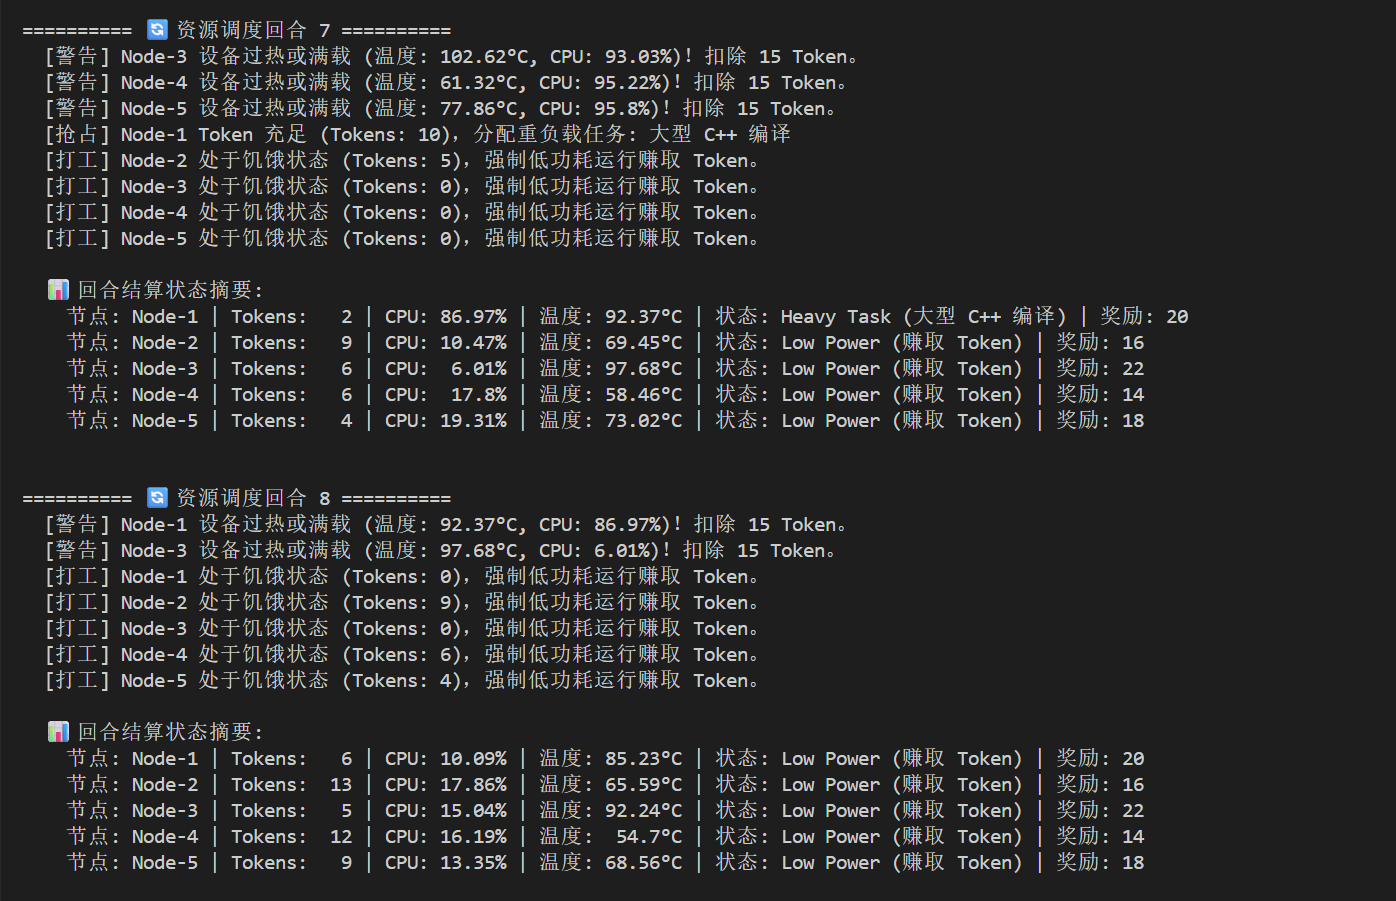
\includegraphics[scale=0.2]{7-8.png}
    \end{minipage}
}
\subfigure[9-10]
{
 	\begin{minipage}[b]{.3\linewidth}
        \centering
        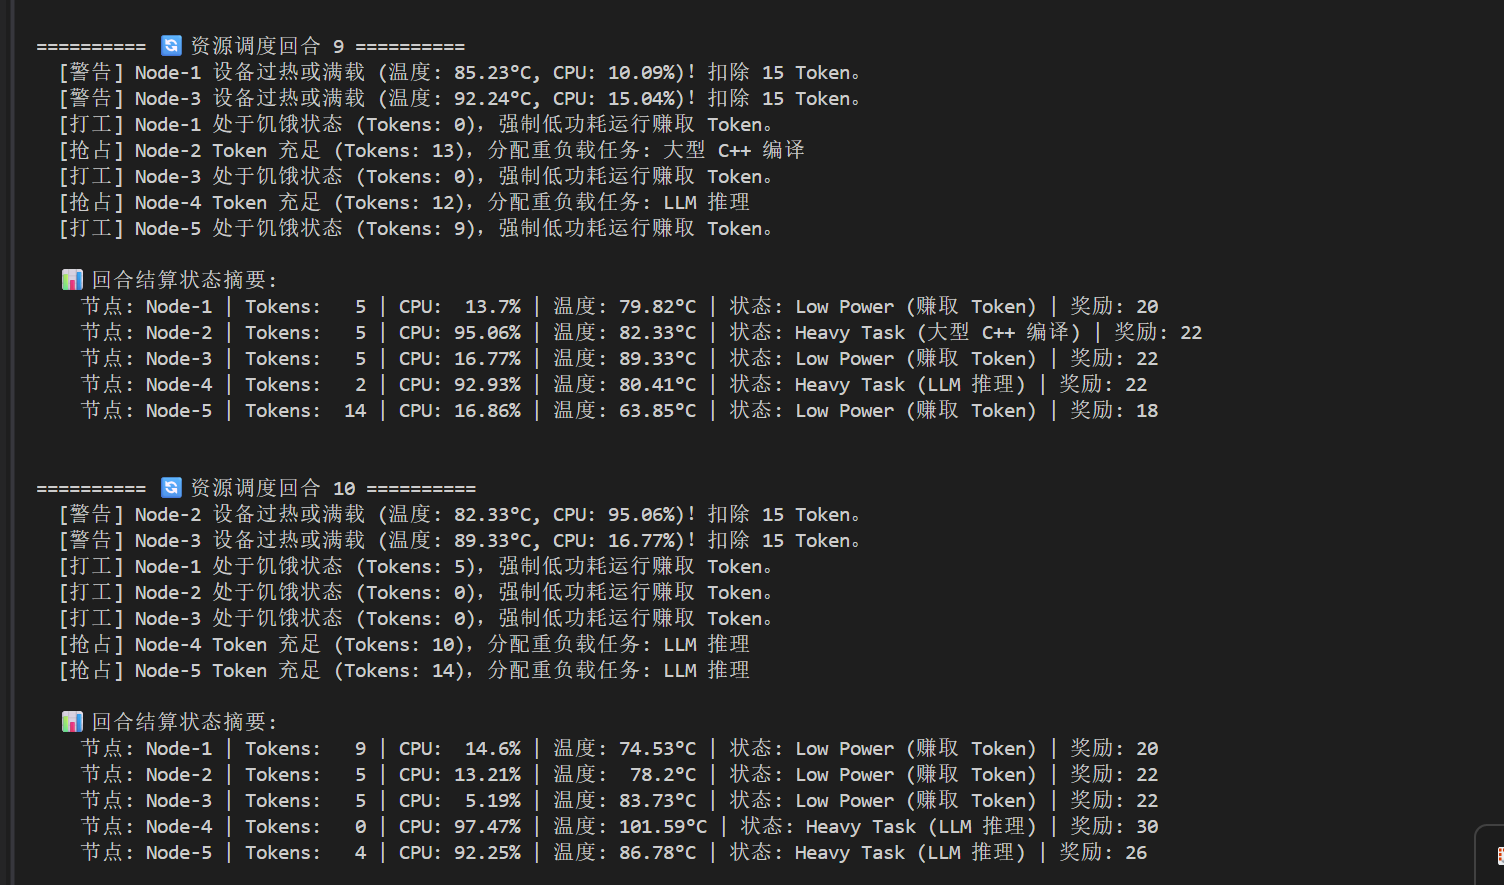
\includegraphics[scale=0.2]{9-10.png}
    \end{minipage}
}
\caption{7-10回合}
\end{figure}

\begin{tcolorbox}[reflectionbox]
通过日志分析，我发现这种看似严苛的“过热惩罚陷入死循环”现象，完美契合了现实世界中老旧操作系统的“过热降频（Thermal Throttling）”策略。热力学中的热量耗散是长尾非线性的，一台被大模型榨干算力的老电脑，不可能在停止任务的瞬间就恢复冰凉。

在这个多 Agent 系统中，电费 Token 本质上起到了“热量缓冲池”的作用。简单的调度器往往会把机器烧毁，而我们引入的这套博弈机制，利用 Token 惩罚强制剥夺了过热设备的任务抢占权，相当于实现了“物理级的强制冷却休眠”。这证明了在分布式异构计算（尤其是性能羸弱的边缘设备）中，引入基于微观经济学（Token 消费）与物理约束（温度监控）相结合的调度策略，远比纯粹追求算力利用率更加安全、健壮。
\end{tcolorbox}

\end{document}